% =============================================================================
% Kapitel 5: Evaluation
% =============================================================================
\chapter{Evaluation}
\label{ch:evaluation}

\todo{Einleitenden Text verfassen. Was wird evaluiert und mit welchem Ziel?}

In der Evaluation wird beschrieben, wie die entwickelten Methoden aus \cref{ch:methodik} auf die in \cref{sec:datengrundlage} beschriebenen Daten angewendet werden und inwiefern die Ergebnisse den Erwartungen entsprechen. Die Evaluation dient dazu -- durch festgelegte Ziele, Kriterien und Messgrößen (\cref{sec:evaluationsdesign}) -- die Modelle in ihrer Fähigkeit zu bewerten, Fahraktivität zuverlässig vorherzusagen. Um das zu erreichen, werden die Modelle auf einer Testumgebung (\cref{sec:testumgebung}) evaluiert und die Ergebnisse (\cref{sec:ergebnisse}) präsentiert. Die Evaluation umfasst sowohl quantitative Gütemaße als auch qualitative Analysen, um ein umfassendes Bild der Leistungsfähigkeit der Modelle zu erhalten. 

% -----------------------------------------------------------------------------
\section{Evaluationsdesign}
\label{sec:evaluationsdesign}

\todo{Das Design der Evaluation beschreiben. Welche Metriken, Kriterien oder Hypothesen werden überprüft?}

Durch verschiedene Darstellungen werden die Gütemaße der Modelle visualisiert, um die Genauigkeit, Stabilität und Verlässlichkeit der Vorhersagen zu bewerten (unter anderem \cref{tab:baselines} und \cref{tab:cv_metrics}). Anhand einer Kreuzvalidierungsmatrix (\cref{fig:cv_matrix}, \cref{fig:cv_matrix_lgbm}, \cref{fig:cv_matrix_lstm_seq} und \cref{fig:cv_matrix_lstm_tab}) wird die Konsistenz der Vorhersagen über verschiedene Datenquellen hinweg überprüft. Da bei den verschiedenen Architekturen fünf Seeds existieren, werden die Gütemaße für die Stabilität gemittelt, um Randwerte zu minimieren. Die Gütemaße werden in \cref{tab:cv_metrics} für alle Modelle und Datenquellen tabellarisch dargestellt, um die Vergleichbarkeit zu erleichtern. Metriken die verwendet werden, sind Accuracy, F1-Score, ROC-AUC, PR-AUC und Brier-Score. Die Kennzahlen werden sowohl für die In-Distribution (auf derselben Datenquelle) als auch für die Out-of-Distribution (auf anderen Datenquellen) berechnet, um die Generalisierungsfähigkeit der Modelle zu bewerten. Accuracy wird als Negativbeispiel für die Limitierungen der Gütemaße diskutiert, da bei stark unausgeglichenen Klassenverteilungen (wie in diesem Anwendungsfall) die Accuracy eine fehlleitende Metrik sein kann. PR-AUC und Brier-Score werden als die wichtigsten Metriken hervorgehoben, da deren Fähigkeit bei unausgeglichen Datensatzen die Qualität der Vorhersagen zu bewerten, besonders relevant ist. Im Laufe der Tests wird eine Ablation der Merkmalsgruppen durchgeführt, um die Bedeutung der einzelnen Merkmale für die Vorhersageleistung zu bewerten (\cref{tab:ablation}). Die Ablation untersucht, wie sich das Entfernen von bestimmten Merkmalsgruppen (Kalender, Lags, Rolling) auf die Metriken auswirkt.

% -----------------------------------------------------------------------------
\section{Testumgebung}
\label{sec:testumgebung}

\todo{Die Testumgebung beschreiben (Hardware, Software, Datensätze, Konfigurationen).}

Bei der Testumgebung handelt es sich um eine standardisierte Umgebung, die sicherstellt, dass die Evaluation reproduzierbar und konsistent durchgeführt werden kann. Zu den Bedingungen gehören folgende Dinge:

\begin{itemize}
    \item Hardware: Die Tests werden auf einem lokalen Computer mit einer NVIDIA GeForce RTX 4070Ti Grafikkarte, 32 GB DDR5 RAM und einem Ryzen 7 9800X3D Prozessor durchgeführt. Die Hardware ist dafür spezialisiert, eine überschaubare Anzahl an anspruchsvollen Aufgaben in kurzer Zeit zu bewältigen, was für die Evaluation der Modelle von Vorteil ist.
    \item Software: Die Softwareumgebung besteht aus Visual Studio Code, Python 3.13 und den folgenden Technologien aus aktuellster Version zum 27.07.2026:scikit-learn, lightgbm, PyTorch, Pandas, Numpy, Angular und TypeScript.
    \item Datensatzkonfiguration: Jede Quelle wird chronologisch im Verhältnis 80/20 in Trainings- und Testteil geteilt. Der Umfang wird je Quelle begrenzt (\texttt{emobpy}: 30 Fahrzeuge, \texttt{ved}: 15 Fahrzeuge aus 4 Dateien, \texttt{yjmob100k}: 50 Personen; \texttt{real\_world\_ev} und \texttt{routine} vollständig), um die Laufzeit beherrschbar zu halten, ohne die Isolationsmatrix zu verändern.
    \item Seeds, Parameter und Kontrollvariablen: Jeder Lauf wird über fünf feste Zufalls-Seeds wiederholt und als Mittelwert samt Standardabweichung berichtet. Die Hyperparameter werden je Modell einmalig festgelegt und über die Isolationsexperimente konstant gehalten, sodass sie zusammen mit dem Feature-Set als Kontrollvariablen wirken.
\end{itemize}

% -----------------------------------------------------------------------------
\section{Ergebnisse}
\label{sec:ergebnisse}

\todo{Die Ergebnisse der Evaluation präsentieren. Tabellen und Grafiken verwenden.}

Bei der Gegenüberstellung des Random Forests mit dem naiven Baseline, zeigt sich in der \cref{tab:baselines}, dass sowohl bei der Metrik PR-AUC als auch bei der missgünstigen Metrik Accuracy, der Random Forest eine bessere Prognose liefert. Die Metrik Majority, die immer behauptet, dass ein Fahrzeug parkt, die Metrik Persistenz-168, welche die Vorwoche überträgt oder Klimatologie, die die Wahrscheinlichkeit zwischen dem Fahren zu einer bestimmten Uhrzeit, an einem Wochentag nimmt, schneiden alle nicht auf dem Niveau des Random Forest ab.

\begin{table}[H]
    \centering
    \caption{Modell (RandomForest) im Vergleich zu naiven Baselines,
    In-Distribution je Datenquelle auf demselben zeitlichen Test-Split.
    Majority = \enquote{immer geparkt}; Persistenz-168 = gleiche Stunde der
    Vorwoche; Klimatologie = $P(\text{fahren}\mid\text{Wochentag},\text{Stunde})$
    aus dem Trainingsteil.}
    \label{tab:baselines}

    \begin{subtable}{\textwidth}
        \centering
        \caption{PR-AUC (Zufalls-Baseline = Aktiv-Rate; höher = besser)}
        \begin{tabular}{lcccc}
            \toprule
            \textbf{Datenquelle} & \textbf{Modell (RF)} & Majority & Persistenz-168 & Klimatologie \\
            \midrule
            emobpy          & \textbf{0,267} & 0,096 & 0,105 & 0,172 \\
            real\_world\_ev & \textbf{0,640} & 0,023 & 0,023 & 0,022 \\
            ved             & \textbf{0,091} & 0,048 & 0,078 & 0,083 \\
            routine         & \textbf{0,884} & 0,264 & 0,672 & 0,797 \\
            yjmob100k       & \textbf{0,683} & 0,382 & 0,478 & 0,489 \\
            \bottomrule
        \end{tabular}
    \end{subtable}

    \vspace{1em}

    \begin{subtable}{\textwidth}
        \centering
        \caption{Accuracy (Majority schneidet durch hohe Aktivitätsrate sehr gut ab)}
        \begin{tabular}{lcccc}
            \toprule
            \textbf{Datenquelle} & \textbf{Modell (RF)} & Majority & Persistenz-168 & Klimatologie \\
            \midrule
            emobpy          & 0,697 & \textbf{0,904} & 0,838 & \textbf{0,904} \\
            real\_world\_ev & \textbf{0,983} & 0,977 & 0,956 & 0,977 \\
            ved             & 0,880 & \textbf{0,952} & 0,919 & \textbf{0,952} \\
            routine         & \textbf{0,898} & 0,736 & 0,887 & 0,868 \\
            yjmob100k       & \textbf{0,726} & 0,618 & 0,659 & 0,619 \\
            \bottomrule
        \end{tabular}
    \end{subtable}
\end{table}


\cref{fig:cv_matrix} stellt die Kreuzvalidierung des Driving-Classifiers mit dem Random Forest Algorithmus dar. Die Matrix zeigt die F1-Scores für jede Kombination von Trainings- und Testdatenquelle. Die Diagonale der Matrix repräsentiert die In-Distribution-Leistung, während Metriken außerhalb der Diagonale die Out-of-Distribution-Leistung darstellen. Die Ergebnisse zeigen, dass die Modelle sich gegenüber dem naive Baseline (majority, persistenz-168, klimatologie) deutlich verbessern. Eine Zeile steht besonders hervor; \texttt{VED} zeigt unter den Datensätzen die geringste Vorhersageleistung, wobei die Datenmenge und Aktivitätsrate mehr als ausreichend sind (\cref{tab:cv_metrics}). Im Anhang in \cref{sec:anhang_abbildungen} befinden sich weitere Kreuzvalidierungsmatrizen mit den übrigen verwendeten Algorithmen.

\begin{figure}[H]
  \centering
  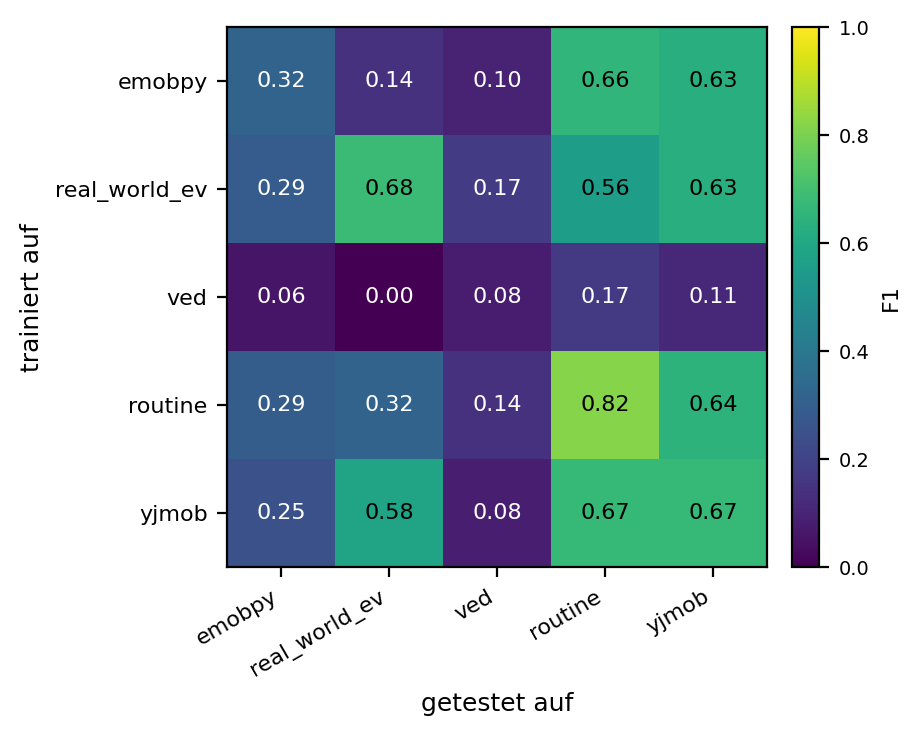
\includegraphics[width=0.85\textwidth]{images/cv_f1_5x5.png}
  \caption{5$\times$5-Kreuzvalidierungsmatrix des Driving-Classifiers
  (RandomForest)}
  \label{fig:cv_matrix}
\end{figure}

\todo{lstm matrizen ansprechen}


\begin{table}[H]
    \centering
    \caption{In-distribution (in eigener Menge -- Datenquelle, in diesem Fall) Gütemaße des Driving-Classifiers je Datenquelle. RandomForest, LightGBM und tab. LSTM-Variante nutzen Merkmalssatz; seq. Variante sieht Rohfenster. \enquote{n.\,z.} = nicht als Trainingsquelle zugelassen, da Quelle Mindestkriterium von 100 Fahrzeugwochen verfehlt (\cref{sec:modellauswahl}).}
    \label{tab:cv_metrics}

    \begin{subtable}{\textwidth}
        \centering
        \caption{RandomForest}
        \label{tab:cv_metrics_rf}
        \begin{tabular}{lcccccc}
            \toprule
            \textbf{Datenquelle} & \textbf{Aktiv-Rate} & Acc. & F1 & ROC & PR & Brier \\
            \midrule
            emobpy          & 0,096 & 0,697 & 0,319 & 0,798 & 0,267 & 0,169 \\
            real\_world\_ev & 0,023 & \textbf{0,983} & 0,681 & 0,884 & 0,640 & \textbf{0,020} \\
            ved             & 0,048 & 0,880 & 0,077 & 0,733 & 0,091 & 0,090 \\
            routine         & 0,264 & 0,898 & \textbf{0,818} & \textbf{0,961} & \textbf{0,884} & 0,073 \\
            yjmob100k       & 0,382 & 0,726 & 0,669 & 0,798 & 0,683 & 0,182 \\
            \bottomrule
        \end{tabular}
    \end{subtable}

    \vspace{1em}

    \begin{subtable}{\textwidth}
        \centering
        \caption{LightGBM}
        \label{tab:cv_metrics_lgbm}
        \begin{tabular}{lcccccc}
            \toprule
            \textbf{Datenquelle} & \textbf{Aktiv-Rate} & Acc. & F1 & ROC & PR & Brier \\
            \midrule
            emobpy          & 0,096 & 0,641 & 0,307 & 0,809 & 0,277 & 0,191 \\
            real\_world\_ev & 0,023 & \textbf{0,969} & 0,366 & 0,850 & 0,256 & \textbf{0,027} \\
            ved             & 0,048 & 0,846 & 0,092 & 0,687 & 0,077 & 0,110 \\
            routine         & 0,264 & 0,880 & \textbf{0,783} & \textbf{0,954} & \textbf{0,873} & 0,090 \\
            yjmob100k       & 0,382 & 0,726 & 0,676 & 0,807 & 0,699 & 0,180 \\
            \bottomrule
        \end{tabular}
    \end{subtable}

    \vspace{1em}

    \begin{subtable}{\textwidth}
        \centering
        \caption{LSTM, tabellarisch (identischer Merkmalssatz)}
        \label{tab:cv_metrics_lstm_tab}
        \begin{tabular}{lcccccc}
            \toprule
            \textbf{Datenquelle} & \textbf{Aktiv-Rate} & Acc. & F1 & ROC & PR & Brier \\
            \midrule
            emobpy          & 0,096 & 0,610 & 0,286 & 0,780 & 0,255 & 0,205 \\
            real\_world\_ev & 0,023 & \multicolumn{5}{c}{n.\,z.} \\
            ved             & 0,048 & \multicolumn{5}{c}{n.\,z.} \\
            routine         & 0,264 & \multicolumn{5}{c}{n.\,z.} \\
            yjmob100k       & 0,382 & 0,726 & 0,676 & 0,806 & 0,703 & 0,180 \\
            \bottomrule
        \end{tabular}
    \end{subtable}

    \vspace{1em}

    \begin{subtable}{\textwidth}
        \centering
        \caption{LSTM, sequenziell (Fenster der letzten 168 Stunden)}
        \label{tab:cv_metrics_lstm_seq}
        \begin{tabular}{lcccccc}
            \toprule
            \textbf{Datenquelle} & \textbf{Aktiv-Rate} & Acc. & F1 & ROC & PR & Brier \\
            \midrule
            emobpy          & 0,096 & 0,661 & \textbf{0,323} & \textbf{0,820} & \textbf{0,288} & 0,194 \\
            real\_world\_ev & 0,023 & \multicolumn{5}{c}{n.\,z.} \\
            ved             & 0,048 & \multicolumn{5}{c}{n.\,z.} \\
            routine         & 0,264 & \multicolumn{5}{c}{n.\,z.} \\
            yjmob100k       & 0,382 & 0,719 & 0,657 & 0,789 & 0,670 & 0,186 \\
            \bottomrule
        \end{tabular}
    \end{subtable}
\end{table}

\begin{table}[htbp]
    \centering
    \caption{Ablation der Merkmalsgruppen: PR-AUC je Datenquelle, zeitlich in-distribution. Verworfene Zeilen richten sich in allen Varianten nach dem vollständigen Merkmalssatz, sodass je Quelle identische Beobachtungen zugrunde liegen.}
    \label{tab:ablation}

    \begin{subtable}{\textwidth}
        \centering
        \caption{RandomForest}
        \label{tab:ablation_rf}
        \begin{tabular}{lccccc}
            \toprule
            \textbf{Variante} & emobpy & real\_world\_ev & ved & routine & yjmob100k \\
            \midrule
            \textbf{voll} (Referenz)     & 0,268 & 0,619 & 0,089 & 0,886 & 0,683 \\
            \addlinespace
            ohne Kalender                & 0,230 & 0,621 & 0,064 & 0,795 & 0,660 \\
            ohne Lags                    & 0,207 & 0,067 & 0,078 & 0,724 & 0,574 \\
            ohne Rolling                 & 0,249 & 0,705 & 0,100 & 0,892 & 0,667 \\
            \addlinespace
            nur Kalender                 & 0,173 & 0,018 & 0,087 & 0,803 & 0,487 \\
            nur Lags                     & 0,207 & 0,669 & 0,094 & 0,793 & 0,670 \\
            nur Rolling                  & 0,134 & 0,187 & 0,048 & 0,253 & 0,497 \\
            \bottomrule
        \end{tabular}
    \end{subtable}

    \vspace{1em}

    \begin{subtable}{\textwidth}
        \centering
        \caption{LightGBM}
        \label{tab:ablation_lgbm}
        \begin{tabular}{lccccc}
            \toprule
            \textbf{Variante} & emobpy & real\_world\_ev & ved & routine & yjmob100k \\
            \midrule
            \textbf{voll} (Referenz)     & 0,277 & 0,177 & 0,074 & 0,861 & 0,698 \\
            \addlinespace
            ohne Kalender                & 0,238 & 0,308 & 0,064 & 0,752 & 0,683 \\
            ohne Lags                    & 0,216 & 0,068 & 0,077 & 0,825 & 0,598 \\
            ohne Rolling                 & 0,261 & 0,625 & 0,122 & 0,871 & 0,690 \\
            \addlinespace
            nur Kalender                 & 0,173 & 0,019 & 0,095 & 0,820 & 0,487 \\
            nur Lags                     & 0,207 & 0,669 & 0,091 & 0,792 & 0,670 \\
            nur Rolling                  & 0,135 & 0,183 & 0,049 & 0,263 & 0,517 \\
            \bottomrule
        \end{tabular}
    \end{subtable}

    \vspace{1em}

    \begin{subtable}{\textwidth}
        \centering
        \caption{LSTM, tabellarischs}
        \label{tab:ablation_lstm_tab}
        \begin{tabular}{lccccc}
            \toprule
            \textbf{Variante} & emobpy & real\_world\_ev & ved & routine & yjmob100k \\
            \midrule
            \textbf{voll} (Referenz)     & 0,259 & 0,504 & 0,099 & 0,582 & 0,701 \\
            \addlinespace
            ohne Kalender                & 0,233 & 0,358 & 0,101 & 0,704 & 0,692 \\
            ohne Lags                    & 0,201 & 0,088 & 0,087 & 0,353 & 0,603 \\
            ohne Rolling                 & 0,256 & 0,567 & 0,101 & 0,598 & 0,691 \\
            \addlinespace
            nur Kalender                 & 0,163 & 0,018 & 0,079 & 0,362 & 0,480 \\
            nur Lags                     & 0,206 & 0,614 & 0,087 & 0,756 & 0,666 \\
            nur Rolling                  & 0,127 & 0,152 & 0,048 & 0,253 & 0,526 \\
            \bottomrule
        \end{tabular}
    \end{subtable}
\end{table}

\todo{memo ablation-interpretation (\cref{tab:ablation}): (1) lags = tragende gruppe -- 'ohne Lags' kostet am meisten (real\_world\_ev -0,552, routine -0,161, yjmob -0,109); 'nur Lags' erreicht fast/über referenz. (2) rolling redundant -- 'ohne Rolling' bei 3/5 quellen BESSER als voll (real\_world\_ev 0,705>0,619, ved 0,100>0,089, routine 0,892>0,886); 'nur Rolling' durchweg am schlechtesten -> rolling bringt gegenüber lags nur rauschen. (3) kalender quellenabhängig: bei routine (regelbasiert) reicht 'nur Kalender' fast (0,803 vs 0,886), bei real\_world\_ev bricht es ein (0,018). LIMITATION: ved durchgehend nahe zufall (aktiv-rate 0,048) -> deltas dort nicht interpretierbar; real\_world\_ev n=1 fahrzeug -> lgbm schwankt 0,177..0,669 = stichprobenrauschen.}
